\documentclass[12pt,]{article}
\usepackage{lmodern}
\usepackage{amssymb,amsmath}
\usepackage{ifxetex,ifluatex}
\usepackage{fixltx2e} % provides \textsubscript
\ifnum 0\ifxetex 1\fi\ifluatex 1\fi=0 % if pdftex
  \usepackage[T1]{fontenc}
  \usepackage[utf8]{inputenc}
\else % if luatex or xelatex
  \ifxetex
    \usepackage{mathspec}
  \else
    \usepackage{fontspec}
  \fi
  \defaultfontfeatures{Ligatures=TeX,Scale=MatchLowercase}
\fi
% use upquote if available, for straight quotes in verbatim environments
\IfFileExists{upquote.sty}{\usepackage{upquote}}{}
% use microtype if available
\IfFileExists{microtype.sty}{%
\usepackage{microtype}
\UseMicrotypeSet[protrusion]{basicmath} % disable protrusion for tt fonts
}{}
\usepackage[margin=1in]{geometry}
\usepackage{hyperref}
\hypersetup{unicode=true,
            pdftitle={Vowel duration and tongue root advancement: Results from an exploratory study of the relation between voicing and vowel duration},
            pdfauthor={Stefano Coretta},
            pdfborder={0 0 0},
            breaklinks=true}
\urlstyle{same}  % don't use monospace font for urls
\usepackage{natbib}
\bibliographystyle{unified}
\usepackage{graphicx,grffile}
\makeatletter
\def\maxwidth{\ifdim\Gin@nat@width>\linewidth\linewidth\else\Gin@nat@width\fi}
\def\maxheight{\ifdim\Gin@nat@height>\textheight\textheight\else\Gin@nat@height\fi}
\makeatother
% Scale images if necessary, so that they will not overflow the page
% margins by default, and it is still possible to overwrite the defaults
% using explicit options in \includegraphics[width, height, ...]{}
\setkeys{Gin}{width=\maxwidth,height=\maxheight,keepaspectratio}
\setlength{\emergencystretch}{3em}  % prevent overfull lines
\providecommand{\tightlist}{%
  \setlength{\itemsep}{0pt}\setlength{\parskip}{0pt}}
\setcounter{secnumdepth}{5}
% Redefines (sub)paragraphs to behave more like sections
\ifx\paragraph\undefined\else
\let\oldparagraph\paragraph
\renewcommand{\paragraph}[1]{\oldparagraph{#1}\mbox{}}
\fi
\ifx\subparagraph\undefined\else
\let\oldsubparagraph\subparagraph
\renewcommand{\subparagraph}[1]{\oldsubparagraph{#1}\mbox{}}
\fi

%%% Use protect on footnotes to avoid problems with footnotes in titles
\let\rmarkdownfootnote\footnote%
\def\footnote{\protect\rmarkdownfootnote}

%%% Change title format to be more compact
\usepackage{titling}

% Create subtitle command for use in maketitle
\newcommand{\subtitle}[1]{
  \posttitle{
    \begin{center}\large#1\end{center}
    }
}

\setlength{\droptitle}{-2em}

  \title{Vowel duration and tongue root advancement: Results from an exploratory
study of the relation between voicing and vowel duration}
    \pretitle{\vspace{\droptitle}\centering\huge}
  \posttitle{\par}
    \author{Stefano Coretta}
    \preauthor{\centering\large\emph}
  \postauthor{\par}
    \date{}
    \predate{}\postdate{}
  
\usepackage{cleveref}
\usepackage{ctable}

\begin{document}
\maketitle

\hypertarget{introduction}{%
\section{Introduction}\label{introduction}}

It is well known that voiced stops (stops generally articulated with
simultaneous vibration of the vocal folds) are almost universally
accompanied by two phonetic correlates: advanced tongue root and
preceding longer vowel durations
\citep{westbury1983, lisker1974, fowler1992}. While a lot of work has
been done on each of these topic separately, less is known about their
relation. In this exploratory study of the articulatory correlates of
stop voicing, it is found that tongue root advancement---a mechanism
known to facilitate voicing during stop closure---is initiated during
the production of the vowel preceding a stop. This replicates previous
work on tongue root position. Moreover, the results of this study
indicate that the acoustic duration of the vowel is positively
correlated with tongue root position, such that longer vowel durations
correspond to greater tongue root advancement.

\hypertarget{tongue-root-position-and-voicing}{%
\subsection{Tongue root position and
voicing}\label{tongue-root-position-and-voicing}}

One of the differences in supra-glottal articulation between voiced and
voiceless stops concerns the position of the tongue root relative to the
front-back dimension of the oral tract. The initiation and maintenance
of vocal fold vibration (i.e.~voicing) requires a difference in air
pressure between the cavities below and above the glottis. Specifically,
the sub-glottal pressure needs to be higher than the supra-glottal
pressure, in other words, there must be a positive transglottal air
pressure differential \citep{berg1958, rothenberg1967}. This property of
voicing is formally known as the Aerodynamic Voicing Constraint
\citep{ohala2011}. When the oral tract is completely occluded during the
production of a stop closure, the supra-glottal pressure quickly
increases, due to the incoming airstream from the lungs. Such pressure
increase can hinder the ability to sustain vocal fold vibration during
closure, to the point voicing ceases.

An articulatory solution to counterbalance the increased pressure is to
enlarge the supra-glottal cavity by advancing the root of the tongue. It
has been repeatedly observed that the tongue root is in a more front
position in voiced stops compared to voiceless stops
\citep{kent1969, perkell1969, westbury1983}. \citet{rothenberg1967}
calculates that the walls of the oral tract can absorb the incoming
airflow for 20 to 30 ms by passive expansion, after which the sub- and
supra-glottal pressures would equalise and voicing cease. Based on these
estimates, a passive expansion of the pharyngeal walls is thus not
sufficient to maintain voicing during the closure of a stop.

Reaching a complete ballistic forward gesture would require the tongue
root about 70 to 90 ms \citep{rothenberg1967}. Given that voiced stop
closures are on average shorter than that (the mean duration is about 64
ms in \citet{luce1985}), it is natural that the movement is initiated
during the production of the vowel, so that an appreciable amount of
advancement is obtained when closure is achieved. Furthermore,
\citet{westbury1983} finds that tongue root advancement is initiated
before the achievement of full closure and that there is a forward
movement even in some cases of voiceless stops, although the rate and
magnitude of the advancement were consistently higher in voiced stops.
Finally, tongue root adjustments seem to target more specifically
lingual consonants, while the tongue body is more involved in labials
consonants \citet{perkell1969, westbury1983}.

However, the relation between tongue root advancement and voicing is a
complex one. First, tongue root advancement is not the only mechanism
for sustaining voicing during a stop
\citep{rothenberg1967, westbury1983, ohala2011} and it has a certain
degree of idiosyncrasy \citep{ahn2016}. Other solutions include
expansion of the lateral walls of the pharynx, larynx lowering
\citep{riordan1980}, opening of the velopharyngeal port
\citep{yanagihara1966}, producing a retroflex occlusion
\citep{sprouse2008}. Second, implementation of tongue root advancement
can be decoupled from the actual presence of vocal fold vibration. In
\citet{westbury1983}, advancement of the tongue root is found in some
productions of voiceless stops, which is counterintuitive given that
tongue root advancement is generally considered to be a feature of
voiced stops. Similarly, \citet{ahn2015, ahn2016, ahn2018} find that the
tongue root is more advanced in the phonologically voiced stops
independent of whether they actually show vocal fold vibration or not.

To summarise, tongue root advancement is a common articulatory solution
employed to counterbalance the increase in supra-glottal pressure and
maintaining voicing during the production of at least lingual voiced
stops. While this gesture is not exclusive of voiced stops and it can be
implemented even in the absence of vocal fold vibration, tongue root
advancement seems to be a robust correlate of (phonological) voicing.

\hypertarget{vowel-duration-and-voicing}{%
\subsection{Vowel duration and
voicing}\label{vowel-duration-and-voicing}}

A great number of studies showed that, cross-linguistically, vowels tend
to be longer when followed by voiced obstruents than when they are
followed by voiceless ones
\citep{house1953, peterson1960, chen1970, klatt1973, lisker1974, farnetani1986, fowler1992, hussein1994, esposito2002, lampp2004, durvasula2012}.
This so-called `voicing effect' has been reported in a variety of
languages, including (but not limited to) English, German, Hindi,
Russian, Arabic, Korean, Italian, and Polish (see
\citealt{maddieson1976} and \citealt{begus2017} for a more comprehensive
list).\footnote{While \citet{keating1984} finds no statistical difference in vowel durations before voiceless vs. voiced stops, \citet{nowak2006} reports a 4.5 ms effect and the data in \citet{malisz2008} suggest an effect of 3.5 ms. \citet{begus2017} argues that the null finding in \citet{keating1984} could be due to low statistical power.}
The existence of the voicing effect is supported by abundant empirical
evidence, although no agreement has been reached regarding its causes
\citep{durvasula2012, soskuthy2013}.

\citet{coretta2018j} presents results on vowel durations in Italian and
Polish based on the acoustic data of the study discussed here. The data
indicates that the raw mean difference in vowel duration before
voiceless vs.~voiced stops in Italian and Polish is about 11.5 and 7.5
ms respectively. Linear mixed modelling suggests an effect of 16 ms (SE
= 4.4) in both languages (see \citealt{coretta2018j} for details).

\hypertarget{this-study}{%
\subsection{This study}\label{this-study}}

To summarise, tongue root advancement and longer vowel durations are two
correlates of voicing (broadly defined). Previous studies have shown
that voicing can be maintained by advancing the tongue root during the
production of voiced stops and that vowels followed by voiced stops tend
to be longer than vowels followed by voiceless stops. The results from
this exploratory study of Italian and Polish show that tongue root
advancement and longer vowel durations are also directly linked in
different ways.

\hypertarget{methodology}{%
\section{Methodology}\label{methodology}}

\hypertarget{participants}{%
\subsection{Participants}\label{participants}}

Participants were recruited in Manchester (UK), and Verbania (Italy)
Eleven native speakers of Italian (5 females, 6 males) and 6 native
speakers of Polish (3 females, 3 males) participated in this study. Most
speakers of Italian are originally from the North of Italy, while 3 are
from Central Italy. The Polish speakers came from different parts of
Poland (2 from the west, 3 from the centre, and 1 from the east). This
study has been approved by the SALC Ethics committee of the University
of Manchester (REF 2016-0099-76). The participants signed a written
consent and received a monetary compensation of £10.

\hypertarget{equipment}{%
\subsection{Equipment}\label{equipment}}

\label{s:equipment}

Simultaneous recordings of audio and ultrasound tongue imaging were
obtained in the Phonetics Laboratory at the University of Manchester
(UK) and in a quiet room in Verbania (Italy). An Articulate Instruments
Ltd™ system was used for this study. The system is made of a TELEMED
Echo Blaster 128 unit, an Articulate Instruments Ltd™ P-Stretch
synchronisation unit, and a FocusRight Scarlett Solo pre-amplifier (see
\Cref{f:uti-setup}). A TELEMED C3.5/20/128Z-3 ultrasonic transducer
(20mm radius, 2-4 MHz) and a Movo LV4-O2 Lavalier microphone were used
respectively for the acquisition of ultrasonic and audio data. The
ultrasonic probe was placed in contact with the sub-mental triangle,
aligned with the mid-sagittal plane. A metallic headset designed by
Articulate Instruments Ltd™ (\citeyear{articulate2008}) was used to hold
the probe in a fixed position and inclination relative to the head. The
acquisition of the mid-sagittal ultrasonic and audio signals was
achieved with the software Articulate Assistant Advanced (AAA, v2.17.2)
running on a Hawlett-Packard ProBook 6750b laptop with Microsoft Windows
7. The synchronisation of the ultrasonic and audio signals was performed
by AAA after recording by means of a synchronisation signal produced by
the P-Stretch unit. The ranges of the ultrasonic settings were: 43-68
frames per second, 88-114 number of scan lines, 980-988 pixel per scan
line, field of view 71-93°, pixel offset 109-263, depth 75-180 mm. The
audio signal was sampled at 22050 Hz (16-bit).

\hypertarget{materials}{%
\subsection{Materials}\label{materials}}

Disyllabic words of the form
C\textsubscript{1}V\textsubscript{1}C\textsubscript{2}V\textsubscript{2}
were used as targets, where C\textsubscript{1} = /p/, V\textsubscript{1}
= /a, o, u/, C\textsubscript{2} = /t, d, k, g/, and V\textsubscript{2} =
V\textsubscript{1} (e.g.~\emph{pata}, \emph{pada}, \emph{poto}, etc.),
giving a total of 12 target words, used both for Italian and
Polish.\footnote{Note that stressed vowels in open syllables in Italian are long \citep{renwick2016}. Moreover, /o/ is used here for typographical simplicity to indicate the mid-back vowels of Italian and Polish, although they do differ in quality. See \citet{kramer2009, renwick2016, gussmann2007}.}
The resulting words are nonce words, with a few exceptions, and they
were presented in the languages' respective writing conventions (see
\Cref{a:targets}). A labial stop was chosen as the first consonant to
reduce possible coarticulation with the following
vowel.\footnote{However, note that \citet{westbury1983} and \citet{vazquez-alvarez2007} report tongue body lowering in the context of labial stops.}
Central/back vowels only were included in the target words for two
reasons. First, high and mid front vowels tend to be difficult to image
with ultrasound, given their greater distance from the ultrasonic probe
when compared with back vowels. Second, high and mid front vowels
usually produce less tongue displacement from and to a stop consonant.
This characteristic can make it more difficult to identify gestural
landmarks using the methodology discussed in \Cref{s:process}. Since the
focus of the study was to explore differences in the closing gesture of
voiceless and voiced stops, only lingual consonants have been included,
since of course the closure of labial stops cannot be imaged with
ultrasound. The sentence \emph{Dico X lentamente} `I say X slowly' in
Italian, and \emph{Mówię X teraz} `I say X now' for Polish functioned as
frames for the test
words.\footnote{Due to software constraints, the Polish frame sentence was presented on screen without diacritics. The speakers read them as if spelled correctly.}
Speakers were instructed to read the sentences without pauses and to
speak at a comfortable pace.

\hypertarget{procedure}{%
\subsection{Procedure}\label{procedure}}

The participants familiarised themselves with the sentence stimuli at
the beginning of the session. Headset and probe were then fitted on the
participant's head. The participant read the sentence stimuli, which
were presented on the computer screen in a random order, while the audio
and ultrasonic signals were acquired simultaneously. The random list of
sentences was read 6 times consecutively (with the exception of IT02,
who repeated the sentences 5 times only). Due to software constraints,
the order of the sentences within participant was kept the same for each
of the six repetitions. The participant could optionally take breaks
between one repetition and the other. Sentences with hesitations or
speech errors were immediately discarded and re-recorded. A total of
1212 tokens (792 from Italian, 420 from Polish) were obtained.

\hypertarget{data-processing-and-statistical-analysis}{%
\subsection{Data processing and statistical
analysis}\label{data-processing-and-statistical-analysis}}

\label{s:process}

The audio data was subject to force alignment using the SPeech
Phonetisation Alignment and Syllabification software (SPPAS,
\citealt{bigi2015}). The outcome of the automatic alignment was then
manually corrected, according to the recommendations in
\citet{machac2009}. The onset and offset of V1 in the
C\textsubscript{1}V\textsubscript{1}C\textsubscript{2}V\textsubscript{2}
test words were respectively placed in correspondence of the appearance
and disappearance of higher formant structure in the spectrogram. Vowel
duration was calculated as the duration of the V1 onset to V1 offset
interval. Speech rate is the number of syllables in the sentence (8 in
Italian and 6 in Polish) divided by the duration of the sentence in
seconds.

The displacement of the tongue root was obtained from the ultrasonic
data according to the procedure used in \citet{kirkham2017}. Smoothing
splines were automatically fitted to the visible tongue contours in AAA.
Manual correction was then applied in cases of clear tracking errors. A
fan-like frame consisting of 42 equidistant radial lines superimposed on
the ultrasonic image was used as the coordinate system. The origin of
the 42 fan-lines coincides with the (virtual) origin of the ultrasonic
beams, such that each fan-line is parallel to the direction of the
ultrasonic scan lines. Tongue root displacement was thus calculated as
the displacement of the fitted spline along a selected vector
\citep{strycharczuk2015}. For each participant, the fan-line with the
highest standard deviation of displacement within the area corresponding
to the speaker's tongue root was chosen as the tongue root displacement
vector. A Savitzky--Golay smoothing filter (second-order, frame length
75 ms) was applied to the raw displacement. Displacement values for
analysis are taken from the smoothed displacement signal. Tongue root
displacement was obtained from a static time point (the onset of the
closure of C2) and along the duration of the vowel. The displacement
values along the vowel duration were extracted at time points
corresponding to real ultrasonic video frames. Given the average frame
rate is 55 frames per second, values are sampled about every 20 ms.

Statistical analysis was performed in R v3.5.2 \citep{r-core-team2018}.
Linear mixed-effects models were fitted with lme4 v1.1-19
\citep{bates2015}. Factor terms were coded with treatment contrasts (the
reference level is the first listed for each factor): C2 voicing
(voiceless, voiced), vowel (/a/, /o/, /u/). Speech rate was centred for
inclusion in the statistical models, by subtracting the mean speech rate
across all speakers from the calculated speech rate values. Centring
ensures the intercepts are interpretable. \emph{t}-tests with
Satterthwaite's approximation to degrees of freedom on the individual
terms were used to obtain \emph{p}-values using lmerTest v3.0-1
\citep{kuznetsova2017, luke2017}. An effect is considered significant if
the \emph{p}-value is below the alpha level (\(\alpha = 0.05\)).
Generalised additive mixed models were fitted with mgcv v1.8-26
\citep{wood2011, wood2017}. The smooths used thin plate regression
splines as basis \citep{wood2003}. The ordered factor difference smooths
method described in \citet{soskuthy2017, wieling2018} was used to model
the effect of factor terms in GAMs. The models were fitted by maximum
likelihood (ML) and autoregression in the residuals was controlled with
a first-order autoregressive model.

Significance testing of the relevant predictors was achieved by
comparing the ML score of the full model with the score of a null model
(in which the relevant predictor is dropped), using the
\texttt{compareML()} function of the itsadug package
\citep{van-rij2017}. A preliminary analysis indicated that including
either language or C2 place of articulation as predictors produced
respective \emph{p}-values above the alpha level, without affecting the
estimates of the other terms. \Cref{s:idio} further discusses the
idiosyncratic behaviour of the tongue root observed between speakers,
which does not seem to pattern in any way with their native language.
For these reasons, these variables were not included in the models
reported here and will not be discussed. Future research is warranted to
ascertain language-related differences and possible effects of place of
articulation.

\hypertarget{open-science-statement}{%
\subsection{Open Science statement}\label{open-science-statement}}

Following recent practices which encourage scientific transparency
\citep{cruwell2018, berez-kroeker2018, roettger2019}, data and analysis
code are available on the Open Science Framework.

\hypertarget{results}{%
\section{Results}\label{results}}

\label{s:results}

\hypertarget{tongue-root-position-at-c2-closure-onset}{%
\subsection{Tongue root position at C2 closure
onset}\label{tongue-root-position-at-c2-closure-onset}}

\begin{figure}
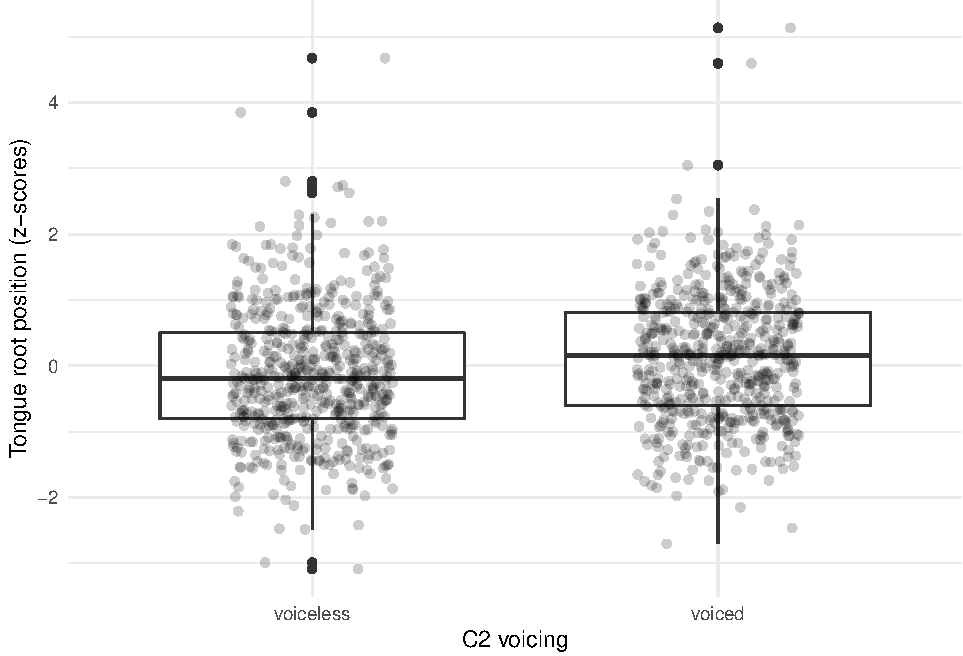
\includegraphics[width=\linewidth]{2018-tra_files/figure-latex/trp-z-box-1} \caption{Fig caption}\label{f:trp-z-box}
\end{figure}

\Cref{f:trp-z-box} shows raw data points and boxplots of the position of
the tongue root at C2 closure onset when C2 is voiceless (left) and
voiced (right). Since the actual value of tongue root position (in mm)
is not informative (it depends on the speaker's anatomy and on the probe
location), scaled tongue root position is used here (note though that
the raw data is used in statistical modelling). The trend is that, not
surprisingly, the position of the tongue root is more advanced if C2 is
voiced compared to its position when C2 is voiceless. A linear
mixed-effects model with tongue root position as the outcome variable
was fitted with the following predictors: fixed effects for C2 voicing
(voiceless, voiced), centred speech rate (as number of syllables per
second, centred), vowel (/a/, /o/, /u/); by-speaker and by-word random
intercepts (a by-speaker random coefficient for C2 voicing led to
singular fit, so was not included in the final model). The effects of C2
voicing and vowel are significant according to \emph{t}-tests with
Satterthwaite's approximation to degrees of freedom. The tongue root at
C2 closure onset is 0.77 mm (SE = 0.35) more front when C2 is voiced,
and it is 1.87 mm (SE = 0.42) more retracted if V1 is /o/.

\hypertarget{tongue-root-position-during-v1}{%
\subsection{Tongue root position during
V1}\label{tongue-root-position-during-v1}}

\label{s:trp-v1}

The position of the tongue root during the articulation of V1 was
assessed with generalised additive mixed models (GAMM). A GAMM was
fitted to tongue root position with the following terms: C2 voicing as a
parametric term; a smooth term over centred speech rate, a smooth term
over V1 proportion with a by-C2 voicing difference smooth, a tensor
product interaction over V1 proportion and centred speech rate; a factor
random smooth over V1 proportion by speaker (penalty order = 1). A
chi-squared test on the ML scores of the full model and model excluding
C2 voicing indicates C2 voicing significantly improves fit (\(\chi\)(3)
= 7.758, \emph{p} = 0.001). \Cref{f:tra-gam} shows that the root
advances during the production of the vowel, relative to its position at
V1 onset. Such forward movement can be seen both in the context of a
following voiced stop and in the one of a voiceless stop. However, the
magnitude of the movement is greater in the former. At V1 offset, there
is a difference in tongue root position of about 1 mm.

\begin{figure}
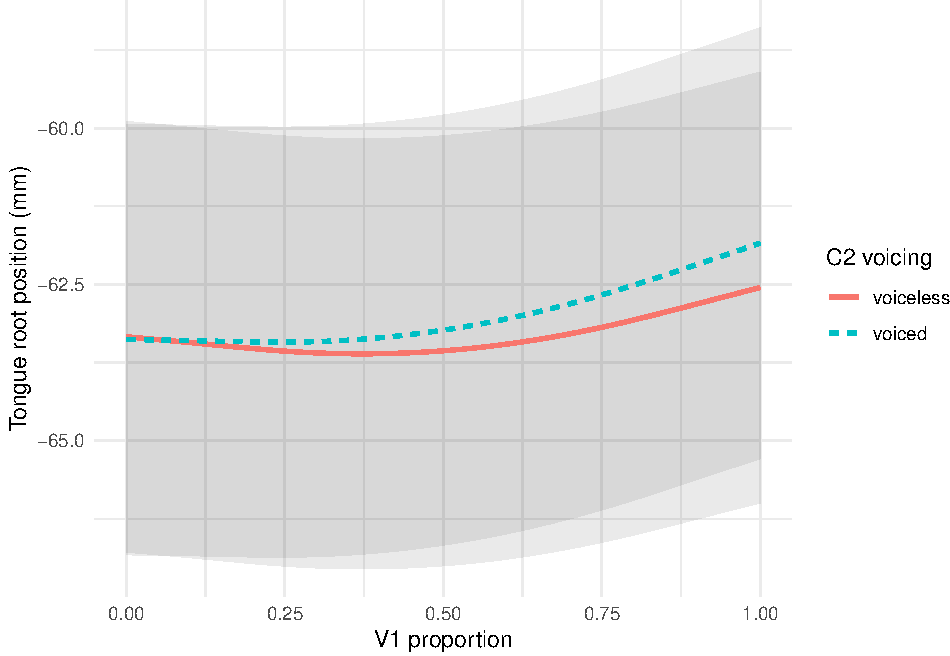
\includegraphics[width=\linewidth]{2018-tra_files/figure-latex/tra-gam-plot, -1} \caption{Fig caption}\label{f:tra-gam-plot, }
\end{figure}

\hypertarget{correlation-between-tongue-root-position-and-v1-duration}{%
\subsection{Correlation between tongue root position and V1
duration}\label{correlation-between-tongue-root-position-and-v1-duration}}

\label{s:trp-vdur}

\begin{figure}
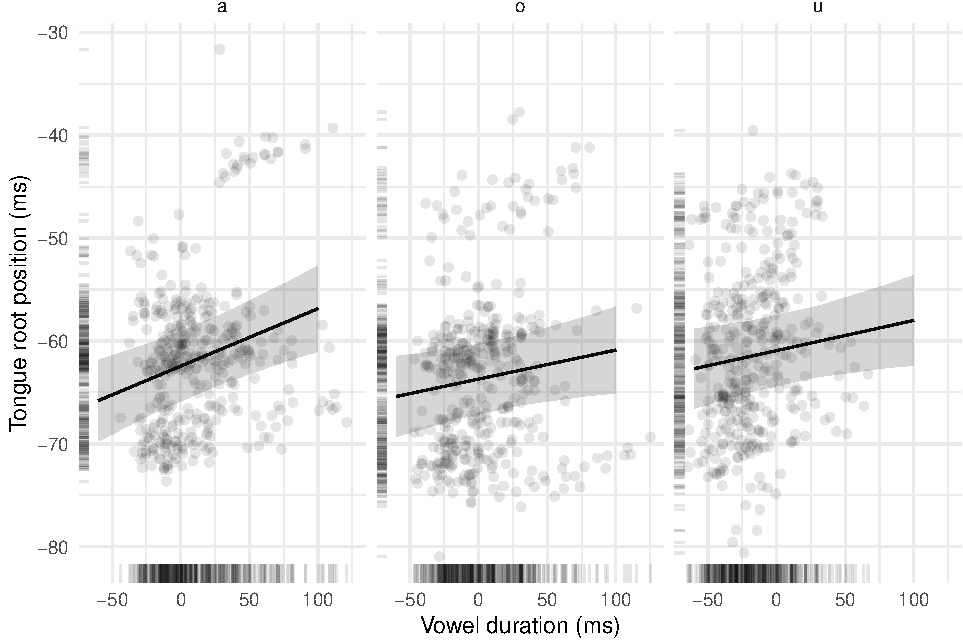
\includegraphics[width=\linewidth]{2018-tra_files/figure-latex/tra-lm-2-plot-1} \caption{Fig caption}\label{f:tra-lm-2-plot}
\end{figure}

A second linear mixed regression was fitted to tongue root position to
assess the effect of V1 duration on root position. The following terms
were included: centred V1 duration (in milliseconds), centred speech
rate (as number of syllables per second), vowel (/a/, /o/, /u/), C2
place of articulation (coronal, velar); an interaction between centred
V1 duration and vowel; by-speaker and by-word random intercept and a
by-speaker random coefficient for V1 duration. All predictors and the V1
duration/vowel interaction are significant. V1 duration and tongue root
position are positively correlated: The longer the vowel, the more
advanced the tongue root is at V1 offset (\(\hat{\beta}\) = 0.056 mm, SE
= 0.015). The effect is stronger with /a/ than with /o/ and /u/ (see
\Cref{f:tra-lm-2-plot}).

\hypertarget{tongue-root-position-during-v2-as-a-function-of-v1-duration}{%
\subsection{Tongue root position during V2 as a function of V1
duration}\label{tongue-root-position-during-v2-as-a-function-of-v1-duration}}

The effect of V1 duration on tongue root position during V1 was modelled
by fitting a GAMM with the following terms: tongue root position as the
outcome variable, smooth terms over V1 duration and V1 proportion, a
tensor product interaction over V1 proportion and V1 duration; a factor
random smooth over V1 proportion by speaker (penalty order = 1). The
full model with the tensor product interaction over V1 proportion and V1
duration has better fit according to model comparison with a model
without the interaction (\(\chi\)(3) = 12.559, \emph{p} \textless{}
0.001). The general trend is that the forward movement of the root
during the vowel is greater the longer the duration of the vowel
(\Cref{f:tra-gam-2-plot}). Moreover, the trajectory curvature increases
with vowel duration: Shorter vowels have a flatter trajectory of tongue
root advancement.

\begin{figure}
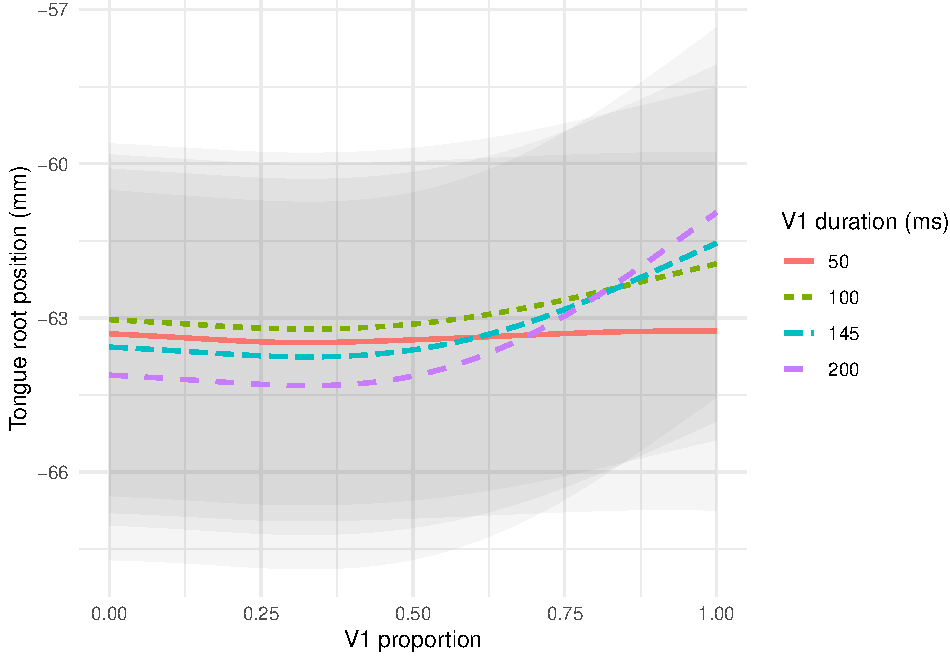
\includegraphics[width=\linewidth]{2018-tra_files/figure-latex/tra-gam-2-plot-1} \caption{Fig caption}\label{f:tra-gam-2-plot}
\end{figure}

\hypertarget{discussion}{%
\section{Discussion}\label{discussion}}

\label{s:discussion}

The results from this exploratory study of voicing and vowel duration in
Italian and Polish suggest there is a more direct relation between
tongue root and vowel duration. Unsurprisingly, the position of the
tongue root at vowel offset if the following stop is voiced is more
front than its position if the following stop is voiceless. This finding
replicates the results in \citet{kent1969, perkell1969, westbury1983},
and \citet{ahn2018}.

However, the data discussed here also suggest that tongue root position
is positively correlated with vowel duration, such that longer vowels
show a more advanced tongue root at vowel offset than shorter vowels.
Said correlation exists independent of the voicing of the consonant
following the vowel. When looking at the position of the tongue root
during the vowel, it was found that the tongue root starts advancing
during the articulation of the vowel. Vowels followed by voiced stops
showed greater tongue root advancement at vowel offset then vowels
followed by voiceless stops, in accordance with the results from the
static analysis at vowel offset. Moreover, a significant interaction
between vowel duration and the trajectory shape was found: Shorter
vowels have a flatter trajectory.

If we take the release of the consonant preceding the vowel as a
reference point, a delayed consonant closure could ensure that, by the
time closure is made, an appreciable amount of tongue root advancement
is achieved, so that the value of the threshold at which transglottal
pressure equalisation is reached and voicing ceases is increased (so
that more time would be required to reach it). This mechanism would
ensure that voicing can be maintained during the duration of the stop
closure.

\citet{coretta2018j} argues that the temporal distance between two
consecutive stop releases in CVCV words of Italian and Polish is not
affected by the voicing of the consonant following the stressed vowel
(the first vowel). The duration of the so-called release to release
interval is stable across voicing contexts. Within this interval, the
timing of the onset of the stop closure produces differences in the
respective durations of vowel and closure. A later closure onset implies
a longer vowel and a shorter closure, while an earlier closure onset
generates a shorter vowel and a longer closure. It is well known that
the closures of voiced stops are longer that those of voiceless stops
\citep{lisker1957, @davis1989}.

As seen in this paper, the closure of voiced stops is initiated later
(relative to the preceding consonant release) compared to the closure of
voiceless stops. Given the temporal stability of the release to release
interval, the delay in producing a full closure seen in the context of
voiced stops has thus a double advantage: (1) A greater degree of tongue
root advancement is achieved at closure onset, and (2) the stop closure
is shorter. Both these features cooperate to satisfy the the aerodynamic
voicing constraint. A more advanced tongue root ensures that the
transglottal pressure differential is sufficient, and a shorter closure
reduces the pressure build-up during the stop closure.

When comparing the effects of vowel duration and speech rate on tongue
root position, though, we face a paradox. Both variables have a positive
effect on tongue root position, so that longer vowels and higher speech
rates imply a more advanced root. However, speech rate has a negative
effect on vowel duration (and segments duration in general), such that
higher speech rates are correlated with shorter vowel durations (this of
course holds for this data, see \citealt{coretta2018j}). If higher
speech rates mean shorter vowels and shorter vowels imply a less
advanced root, we should also find less advancement with higher speech
rates. However, the results indicate the opposite: With higher speech
rates there is more root advancement. A solution to the paradox would be
for the tongue root to be already in a more advanced position at
\emph{vowel onset} when the speech rate is high. Indeed, this is what a
regression model on the vowel onset data suggests. Speech rate is
positively correlated with tongue root position at vowel onset.

While the patterns observed in this study are in agreement with previous
work, the correlation between tongue root position and vowel duration
needs to be replicated in studies which expand the enquired contexts to
other types of consonants and vowels. Investigating the relative phasing
of tongue root and body gestures in lingual and labial consonants is
also necessary to shed light on the mechanisms that could underlie the
timing of stop closures. The following sections further discuss in some
details the idiosyncratic patterns observed across individual speakers
and the estimated value of the difference in tongue root position.

\hypertarget{individual-differences}{%
\subsection{Individual differences}\label{individual-differences}}

\label{s:idio}

\begin{figure}

{\centering 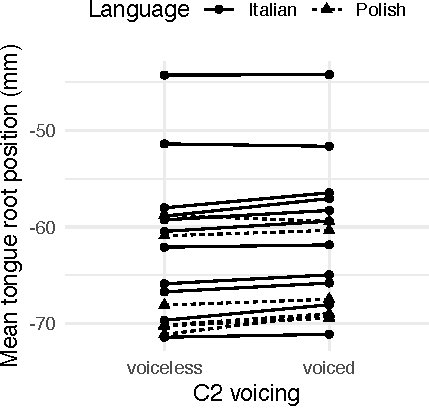
\includegraphics[width=.49\linewidth]{2018-tra_files/figure-latex/trp-voicing-plot-1} 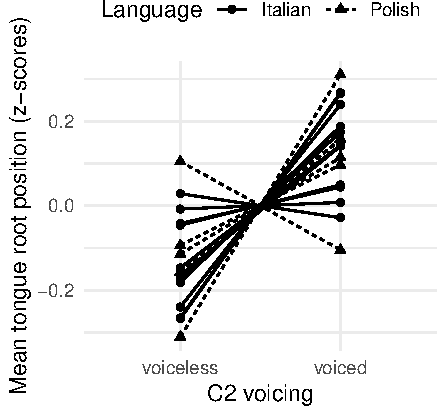
\includegraphics[width=.49\linewidth]{2018-tra_files/figure-latex/trp-voicing-plot-2} 

}

\caption{Fig caption}\label{f:trp-voicing-plot}
\end{figure}

The results presented in \Cref{s:results} and discussed in
\Cref{s:discussion} are general patterns that can be attributed to a
population as inferred from the present sample. However, the data shows
a great amount of individual differences. \Cref{f:trp-voicing-plot}
shows two slope plots of mean tongue root position depending on C2
voicing for each speaker. In each plot, the two means of each speaker
are linked by a line that shows the difference (or lack thereof) in
means. Solid lines are Italian speakers, while dashed lines are Polish
speakers. The \emph{y}-axis of left plot is raw mean positions in
millimetres, while that of the right plot is the standardised values
(z-scores). An upward-slanted slope line indicates that the mean tongue
root position in the voiced condition is higher, while a
downward-slanted slope means a decrease in mean root position. A flat
slope suggests there is no difference in means between the voiceless and
the voiced condition. These plots show that all three possibilities of
slope direction are found in the data. The mean value of tongue root
position with a voiced C2 relative to the voiceless mean is greater in
some speakers, smaller in others, and very similar in yet other
speakers. Moreover, no discernible pattern can be found between the two
languages: Speakers of both languages show more or less the same range
of variation. However, as we have seen in \Cref{s:results}, the
estimated overall effect of C2 voicing is a more advanced tongue root.
The right plot of \Cref{f:trp-voicing-plot} confirms this point
visually. Two speaker show a declining slope (one is Italian and the
other Polish), one has a virtually flat slope, while all the others have
an increasing slope at varying degrees. The individual variation across
speakers found in this data is comparable to that in \citet{ahn2018}.

\begin{figure}
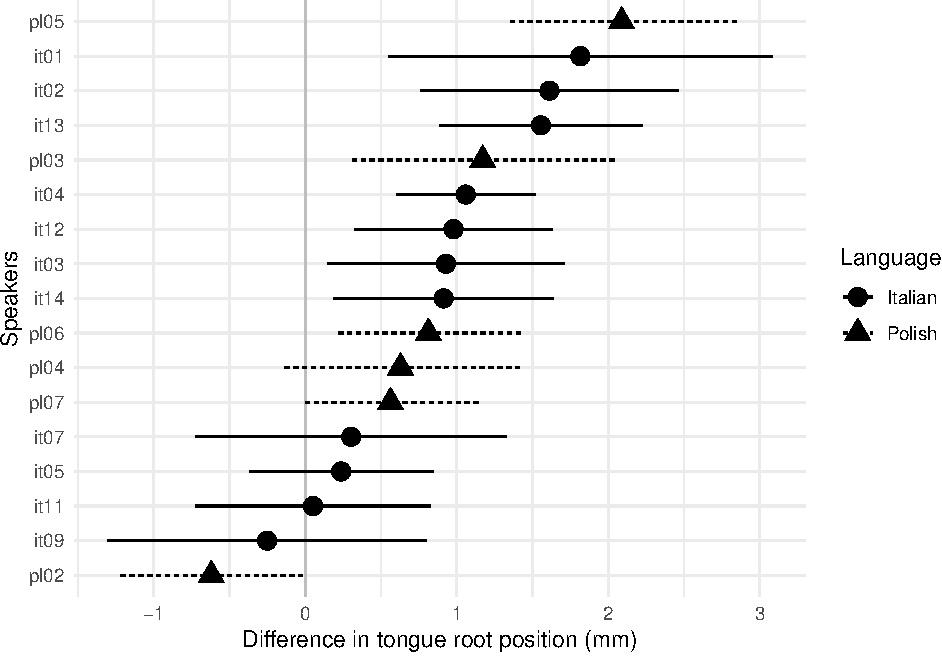
\includegraphics[width=\linewidth]{2018-tra_files/figure-latex/trp-difference-1} \caption{Fig caption}\label{f:trp-difference}
\end{figure}

\Cref{f:trp-difference} shows the mean difference in tongue root
position at vowel offset for each speaker. The horizontal lines indicate
the difference standard error. The bottom 7 speakers (3 Polish, 4
Italian) show either a weak negative difference (the tongue root is
slightly more advanced in voiceless stops) or a weak positive difference
with wide standard errors which include 0. The remaining 11 speakers
have a more robust positive difference (the tongue root is more advanced
in voiced stops). Finally, speakers of each language do not cluster
together, reiterating the observation above that language does not seem
to be an informative parameter.

Interesting individual patterns can also be seen in the trajectories of
tongue root position. \Cref{f:tra-gam-s-ar-plot} shows these
trajectories for the 17 speakers (note that the \emph{y}-axis of each
plot is on a different scale, so magnitude comparisons should not be
made visually). Speakers IT01, IT03, and PL04 in particular have a
somewhat categorical distinction in tongue root position during vowels
followed by voiceless vs.~voiced stops. Such tongue root distinction is
implemented across the total duration of the vowel, rather than towards
the end (as suggested by the results from the aggregated data, see
\Cref{s:trp-v1}). The phonological literature reports cases in which the
tongue root distinction in vowels is enhanced, leading to phonological
alternations or diachronic loss of the voicing distinction with
maintenance of the tongue root distinction (see \citet{vaux1996} and
references therein). The ultrasound data from this study offers
articulatory evidence for a possible precursor of said phonological
patterns.\footnote{All the examples in \citet{vaux1996} are on vowels \textit{following} voiceless vs. voiced stops, rather than preceding, as in the current study. While beyond the scope of this paper, whether this is a systematic gap or not and how this relates to the present findings should be examined in future studies.}

\begin{figure}
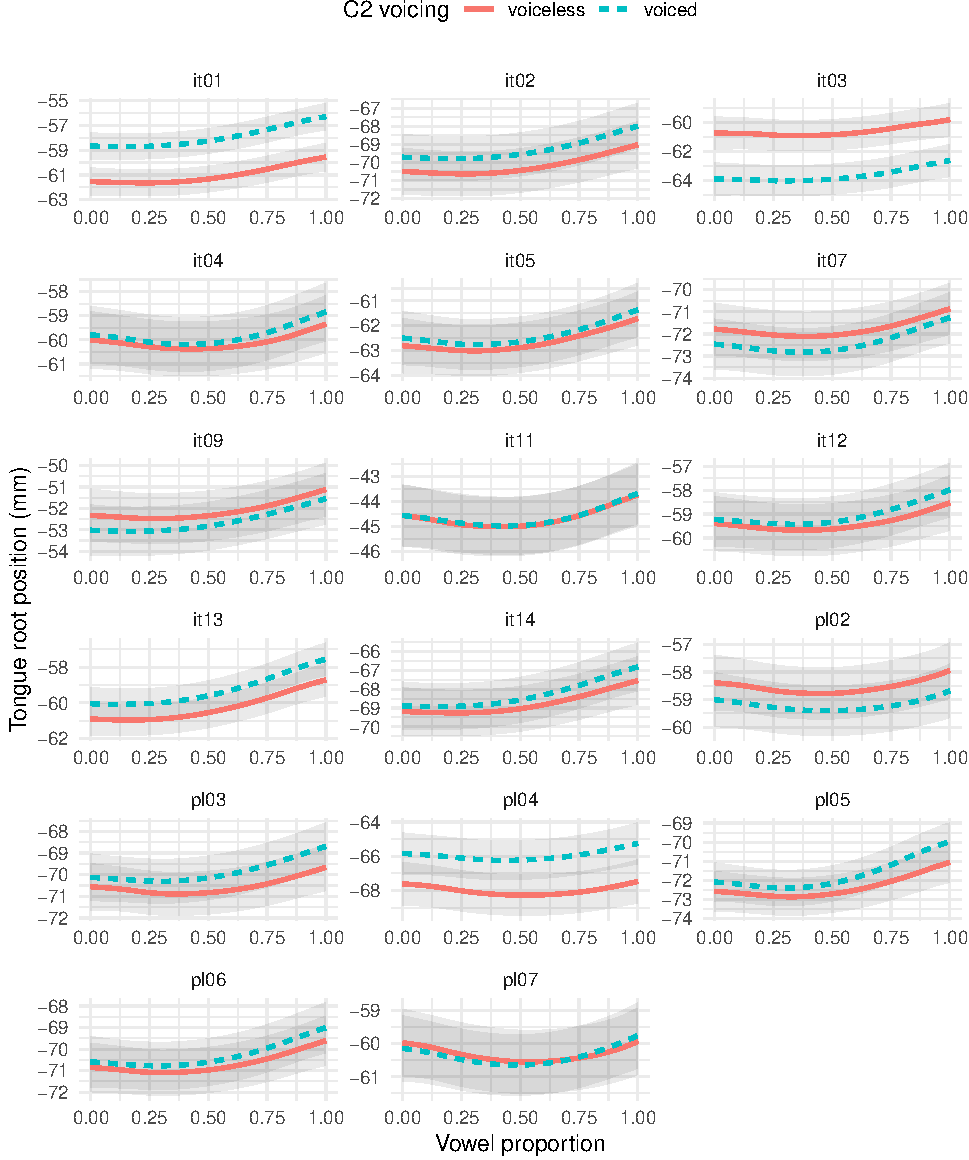
\includegraphics[width=\linewidth]{2018-tra_files/figure-latex/tra-gam-s-ar-plot-1} \caption{Fig caption}\label{f:tra-gam-s-ar-plot}
\end{figure}

\hypertarget{estimates-of-tongue-root-displacement}{%
\subsection{Estimates of tongue root
displacement}\label{estimates-of-tongue-root-displacement}}

It is worth to briefly discuss the estimated difference in tongue root
position between voiceless and voiced stops and its significance. The
estimated magnitude of such difference is 0.77 mm (SE = 0.35). The 95\%
confidence interval for the difference is approximately within the range
0-1.5 mm. \citet{rothenberg1967} argues that the anterior wall of the
lower pharynx (corresponding to the tongue root) can move by 5 mm along
the antero-posterior axis. Figure 1 in \citet{kirkham2017} suggests that
the tongue root of a Twi speaker is about 4 mm more front in /e/ (a +ATR
vowel) than in /ɛ/ (a -ATR vowel). Given that a difference of 4 mm can
produce a substantially different acoustic output in vowels (like two
different phonemes), a smaller difference in tongue root position as
driven by consonantal factors makes
sense.\footnote{Thanks to Sam Kirkham for bringing this point to my attention.}
Moreover, the data presented here indicate that for every millisecond
increase in vowel duration there is a 0.056 mm increase in tongue root
advancement (see \Cref{s:trp-vdur}). If a maximal ballistic forward
movement of the tongue root takes between 70 and 90 ms
\citep{rothenberg1967}, we can estimate a maximum displacement of 3.9 to
5 mm. These values are well in accordance with the maximum possible root
displacement of 5 mm given by Rothenberg.

The results also shed some light on timing aspects of tongue root
advancement. Possibly, the correlation between tongue root position and
vowel duration is a consequence of the timing of the advancement
gesture. In order to obtain such correlation, the onset of the gesture
(during the articulation of the vowel) should be at a fixed distance
from an earlier reference point (like the vowel onset or the preceding
consonant offset) such that the timing of consonant closure will create
the correlation seen in the data. Although ideally the timing of the
onset of the advancing gesture should be fixed, the velocity of the
gesture itself could be different depending on the voicing of the
following consonant. It is possible that the velocity will be greater in
the context of voiced stops, especially if the advancing gesture in this
context is executed with greater muscular force. Unfortunately, a
preliminary screening of the current data on this matter was
inconclusive due to the difficulty in identifying the onset of the
advancing gesture. Further data should be collected with the aim of
testing the hypothesis that the timing of the gesture onset should be
the same in voiceless and voiced contexts, while the velocity of the
gesture should differ in the two contexts.

\hypertarget{conclusion}{%
\section{Conclusion}\label{conclusion}}

\appendix

\hypertarget{target-words}{%
\section{Target words}\label{target-words}}

\label{a:targets}

See \Cref{t:targets}.

\ctable[caption = The list of Italian and Polish target words. An asterisk indicates a real word.,
label = t:targets,
star,
doinside = \footnotesize
]{lllllll}{}{
\FL
Italian   &        &      & \hspace{0.5cm} & Polish &      &      \NN
\cmidrule{1-3}\cmidrule{5-7}
pata      & poto*  & putu & & pata   & poto & putu \NN
pada      & podo   & pudu & & pada*  & podo & pudu \NN
paca*     & poco*  & pucu & & paka*  & poko & puku \NN
paga*     & pogo   & pugu & & paga   & pogo & pugu \LL
}

\bibliography{linguistics}


\end{document}
